\newpage
% ---------------------------------------------------------------------------
\section{Hepburn System}\jsec{ヘボン式}
%[o] LABEL
\label{sec:Hepburn}
\label{sec:HepburnSystem}
\label{sec:OlderHepburnSystem}
\label{sec:NewerHepburnSystem}
% [o] INDEX
\ifor{Hepburn system}{ヘボン式}{へぼんしき}{Hepburn System}
\ifor{Hepburn system!older}{標準ヘボン式ローマ字}{ひょうじゅん・へぼん・ろまあじ}{Hepburn System!altes}
\ifor{Hepburn system!newer}{修正ヘボン式ローマ字}{しゅうせい・へぼんしき・ろうまじ}{Hepburn System!neueres}
\ithree{James Curtis Hepburn}{James Curtis Hepburn}{James Curtis Hepburn}

\newcommand{\lhepburnsystem}{\ivoc{Hepburn system}{ヘボン式}{へぼんしき}{Hepburn System}}
\newcommand{\loldhepburnsystem}{\ivoc{old Hepburn system}{標準ヘボン式ローマ字}{ひょうじゅん・へぼん・ろまあじ}{altes Hepburn System}}
\newcommand{\lnewhepburnsystem}{\ivoc{new Hepburn system}{修正ヘボン式ローマ字}{しゅうせい・へぼんしき・ろうまじ}{neues Hepburn System}}

\begin{wrapfigure}{r}{0.3\textwidth}
        %\raisebox{-.47\height}{
        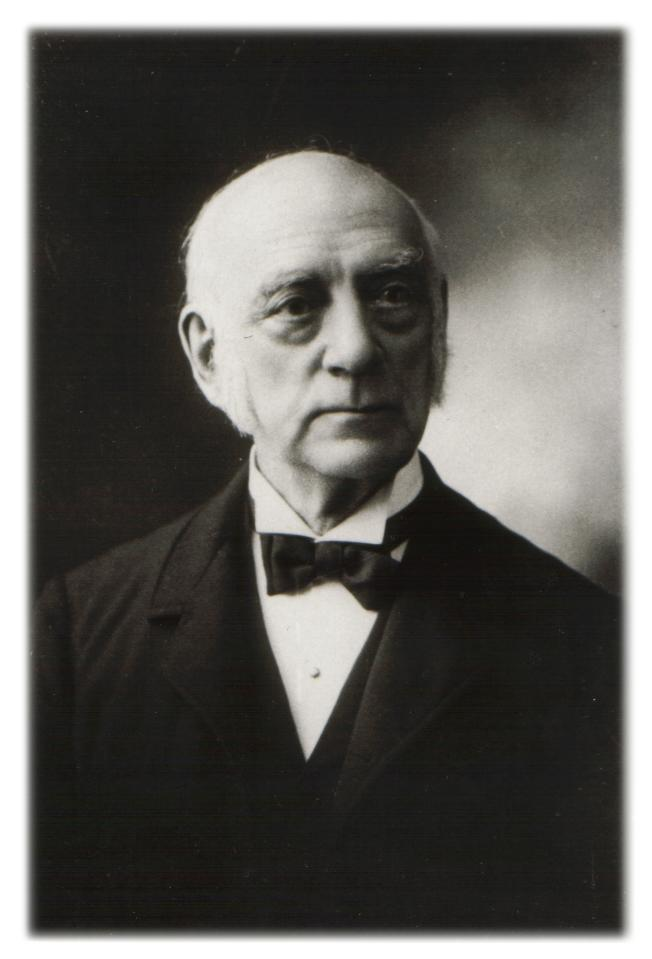
\includegraphics[scale=0.5,trim= 00 00 00 00]{../share/ei/James_Curtis_Hepburn.jpg}%}
        \caption{J. C. Hepburn}
        \label{fig:JamesCurtisHepburn}
\end{wrapfigure}

The \lhepburnsystem{} is one of the two most important transcription systems
for the Japanese written \hyperref[sec:Mora]{morae} based language. The
\textbf{Hepburn system} is the most used system worldwide and in Japan.

The word {ヘボン} /hebon/ is an old writing of the name \textbf{Hepburn}. James
Curtis Hepburn was a US American physician, translator, educator and a
Christian missionary, who used the transcription system in his first Japanese
English Dictionary (3rd ed.) in 1867.

There are mainly two different variants: The \loldhepburnsystem{} variant,
which is used for signs at train stations. And the newer variant the
\lnewhepburnsystem{} which is used as a revised system since 1954 in Kenkyusha
dictionaries. Most western scientists are using this system. This system is
also used in this book.

The \textbf{Hepburn system} uses English orthography to phonetically transcribe
sounds.  Even though the Japanese government prefers the
\hyperref[sec:Kunrei]{kunrei system}, the most popular way of transcribing
Japanese is still the \textbf{Hepburn system}. This is partly because the
\textbf{Hepburn system} creates more accurate results in pronunciation for
speakers of Romance languages, when encounter unfamiliar words, than other
transcription systems, like the \hyperref[sec:Kunrei]{kunrei system} or the
\hyperref[sec:Kunrei]{Nihonshiki}.

The \textbf{new Hepburn system} from 1954, also called \textit{modfied} or
\textit{revised Hepburn}, uses /n/ before certain consonants (the old system
often used /m/: old /shimbashi/, new /shinbashi/). The system is used by the
Kenkyusha's New Japanese-English Dictionary and adopted by the Library of
Congress in 1989.  The \textbf{new Hepburn system} also uses a \textit{macron},
a line above a character that is pronounced longer, if the vowels are part of
the same morpheme: ā, ū, ē, ō. Be aware that ō can stand for おお/オー or
おう/オウ and thus the only drawback of the \textbf{Hepburn system}, while the
pronunciation is correct one has to remember the spelling. However this is
comparatively easy. Some books also placing a \textit{macron} over the /i/.
That is sometimes difficult to distinguish and not part of the \textbf{new
Hepburn system}.\medskip

\begin{tabular}{r|l|l}
        &\textbf{separate morpheme}&\textbf{same morpheme}\\\hline
        aa&邪悪 【じゃあく】 jaaku (evil)& お母さん 【おかあさん】 okāsan (mother)\\
        oo&小躍り【こおどり】 koodori (joy dance)& 大きい 【おおきい】 ōkii (big)\\
        ou&小歌 【こうた】kouta (Muromachi era short song)& 勉強 【べんきょう】benkyō (study)\\
\end{tabular}
\medskip

The \textbf{new Hepburn system} is also used in this book to transcribe Japanese.

%\Link \href{https://en.wikipedia.org/wiki/James_Curtis_Hepburn}{Hepburn}
%\Link \href{https://en.wikipedia.org/wiki/Hepburn_romanization}{Hepburn romanization}

